\chapter{Michelson Morley}
\label{sec:MichelsonMorley}

I 1887 publicerede de to amerikanske fysikere Albert A. Michelson og Edward W. Morley resultaterne af hvad der sidenhen er blevet kendt som Michelson-Morley eksperimentet.

\begin{wrapfigure}{i}{0.5\textwidth}
	\vspace{-10pt}
	\centering
		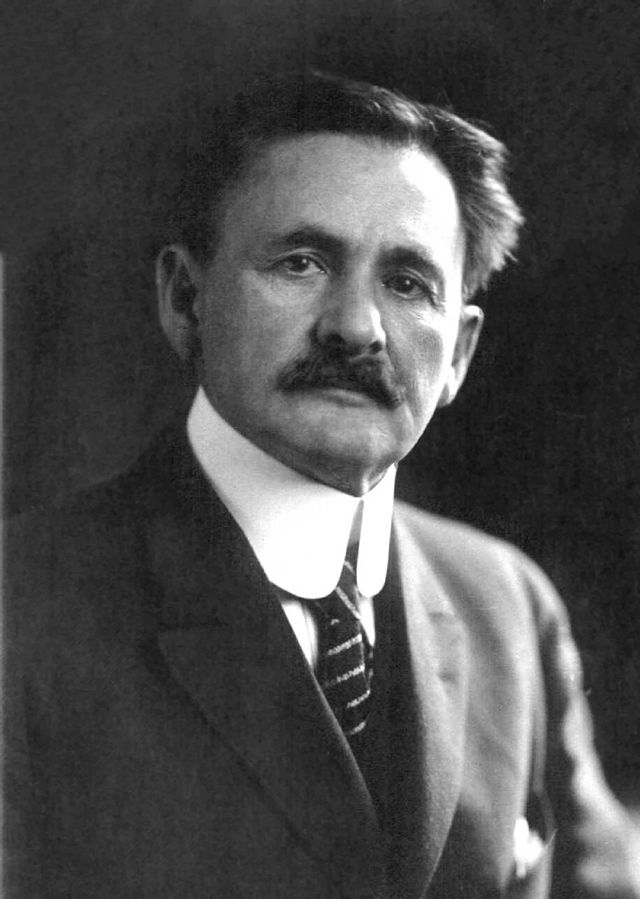
\includegraphics[width=.45\textwidth]{Michelson}
		\caption{Albert A. Michelson}
	\vspace{-10pt}
\end{wrapfigure}
De to fysikere fors�gte at p�vise eksistensen af et medium hvor i lys kunne udbredes. Deres ide var som de fleste andre naturvidenskabs folk p� dette tidspunkt at tolke lys som et b�lgef�nomen. Da vi fra b�lgernes verden ved at b�lger som f.eks. lyd kr�ver et medium at udbredes i f.eks. luft. S� m�tte lys der jo var elektromagnetiske b�lger ligeledes kr�ve et medium at udbredes i. Mediet blev kaldt \emph{�teren}. De pr�vede alts� at detektere en relativ bev�gelse af stof gennem den station�re �ter. Deres forventede resultat udeblev og deres m�linger antages idag for at v�re et st�rkt bevis for at �terteorien ikke var korrekt, ligeledes blev det start skuddet til den forskning som ledte frem til udviklingen af den specielle relativitetsteori, hvori �ter teorien ikke spiller nogen rolle.

\begin{wrapfigure}{i}{0.5\textwidth}
	\vspace{-10pt}
	\centering
		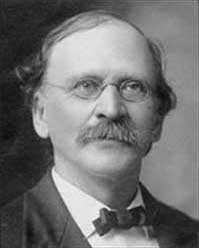
\includegraphics[width=.45\textwidth]{Morley}
		\caption{Edward W. Morley}
	\vspace{-10pt}
\end{wrapfigure}
�teren er med andre ord et hypotetisk medium, hvori elektromagnetisk str�ling som lys kan udbredes. If�lge �terteorien ville lysets hastighed i forhold til Jorden variere p� grund af Jordens bev�gelse gennem �teren. F.eks. ville lyshastigheden v�re mindst, n�r Jorden bev�ger sig i samme retning som lyset, og st�rst n�r Jorden bev�ger sig i modsat retning af lyset.

Michelson og Morley desdignede et fors�g hvor en lysstr�le sendes fra en lyskilde parallelt med Jordens bev�gelsesretning gennem et halvgennemsigtigt spejl, s�ledes at lysstr�len deles i to. Den ene del af lyset sendes direkte gennem spejlet til et nyt spejl hvor det reflekteres tilbage til det halvgennemsigtige spejl.
